\documentclass[tikz,border=2pt]{standalone}
% shared tikz preamble for generating svg figures
% keep this file minimal; figure-specific styles can live in the figure .tex if needed
\usepackage{tikz}
\usetikzlibrary{positioning}
\usetikzlibrary{shapes.geometric}
\usetikzlibrary{arrows}
\usetikzlibrary{decorations}
\usetikzlibrary{decorations.markings}

\tikzset{>=latex}
\tikzstyle{Arrow} = [->, thin, preaction = {decorate}]
\tikzstyle{cor} = [-, dotted, preaction = {decorate}]

\usetikzlibrary{arrows.meta}
\begin{document}
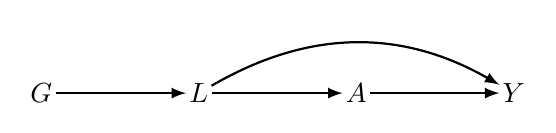
\begin{tikzpicture}
\node [draw=none, inner sep=1] (G) at (0, 0) {$G$};
\node [draw=none, inner sep=1] (L) at (2, 0) {$L$};
\node [draw=none, inner sep=1] (A) at (4, 0) {$A$};
\node [draw=none, inner sep=1] (Y) at (6, 0) {$Y$};
\draw [-latex, thick] (G) to (L);
\draw [-latex, thick] (L) to (A);
\draw [-latex, thick, bend left=30] (L) to (Y);
\draw [-latex, thick] (A) to (Y);
\end{tikzpicture}
\end{document}
